% !TEX root =  podc-submission.tex

\section{Reducing Space Usage}
\label{reducing}

In our implementation, an operation remains in the \nf{blocks} arrays forever. 
Thus, the space used is proportional to the number of operations that have been invoked.
Now, we sketch a mechanism to remove blocks that are no longer needed to use space
polynomial in $p$ and $q$, while maintaining polylogarithmic (amortized) step complexity.  For lack of space, details are in Appendix~\ref{reducing-details}.

We replace the \fld{blocks} array in each node by a red-black tree (RBT)
that stores the blocks.
Each block has an additional \fld{index} field
that represents its position within the original \fld{blocks} array, and
blocks in a RBT are sorted by \fld{index}.
Accessing the block in entry $i$ in the \fld{blocks} array can then be 
replaced by searching the RBT for the block with index $i$.
The attempt to append a new block in entry $i$ of the \fld{blocks} array on line \ref{cas}
is replaced by an attempt to insert a new block with index $i$ into the RBT.
 
Known lock-free search trees have step complexity that includes a term linear in $p$ \cite{EFHR14,Ko20}.  
However, we do not require all the standard search tree functions.
Instead of a standard insertion, we allow a \op{Refresh}'s insertion to fail if another
concurrent \op{Refresh} succeeds in inserting a node, just as the CAS on line \ref{cas}
can fail if a concurrent \op{Refresh} does a successful CAS.
Thus, we can use a particularly simple concurrent RBT implementation.
A sequential RBT can be made persistent using the classic node-copying technique of 
Driscoll et al.~\cite{DSST89}:  all nodes are immutable, and operations on the 
tree are performed by making a new copy of each node $v$ that must be modified, as well
as each node along the path from the root to $v$.
The tree reachable from the new copy of the root is the result of applying the tree operation.
This only adds a constant factor to the running time of any routine designed for a (sequential) RBT.
Once a process has performed an update to the RBT representing the blocks of a node 
$v$ in the tournament tree, 
it uses a CAS to swing $v$'s pointer from the previous RBT root to the new RBT root.
A search in the RBT can simply read the pointer to the RBT root and perform a standard
sequential search on it.
Bashari and Woelfel ~\cite{DBLP:conf/podc/BashariW21} used persistent red-black trees in a similar way to implement a snapshot data structure.

To prevent RBTs from growing without bound, we would like to discard
blocks that are no longer needed.
Ensuring the size of the RBT is polynomial in $p$ and $q$ will 
also keep the running time of our operations polylogarithmic.
We msut keep a block $B$ if any element enqueued by the operations in $E(B)$ has
not yet been dequeued, since a later dequeue may need to traverse the block to 
find its response.
Because of the FIFO nature of queues, this means that we can throw away 
blocks whose indices are smaller than the block containing the oldest enqueue whose
value is still in the queue.
Fortunately, there is an efficient \op{Split} operation that can remove
all nodes with indices less than a given threshold from an RBT in logarithmic time \cite[Sec.~4.2]{Tar83}.

To maintain good amortized time per operation, we periodically do a garbage collection (GC) phase.
After every $p^2$ successful insertions into the RBT representing $\var{root}.\fld{blocks}$,
processes cooperate to perform \op{Split} operations on all nodes of the tournament tree  
to discard unneeded blocks.
We keep an array $\var{last}[1..p]$ where each process writes the index of the last block in
\var{root} that it dequeued an element from.
If a process performing a \op{Refresh} on the root finds that $root.\head$ is a multiple
of $p^2$, it does GC by first helping all pending dequeue operations by other processes,
then reading $\var{last}[1..p]$.

\here{need to complete the description of GC}

Each process takes $\tilde{O}(p)$ to run GC.\footnote{We use $\tilde{O}$ notation
to omit polylogarithmic factors; see Appendix \ref{reducing-details} for precise bounds.}
Since all processes may run GC,
a total of $\tilde{O}(p^2)$ steps is spent on a GC phase.
Between two of these GC phases, there are at least $p^2$ operations, so
GC contributes only $\tilde{O}(1)$ steps per operation in an amortized sense.


\paragraph{Garbage Collection}
We did not handle garbage collection: \nf{Enqueue} operations  remain in the nodes even after their elements have been dequeued.
We can keep track of the \nf{block}s in the \nf{root} whose operations are all terminated, i.e., all enqueues have been dequeued, and the responses of all dequeues have been computed. We call these blocks \it{finished blocks}. If we help the operations of all processes to compute their responses, then we can say if block $B$ is finished, then all blocks before $B$ are also finished. Knowing the most recent finished block in a node, we can reclaim the memory taken by finished blocks. We cannot use arrays (or vectors) to throw the garbage blocks away. We need a data structure that supports \nf{tryAppend()}, \nf{read(i)}, \nf{write(i)} and \nf{split(i)} operations in $O(\log n)$ time, where \nf{split(i)} removes all the indices less than~\nf{i}. If each process tries to do the garbage collection once every $p^2$ operations on the queue, then the amortized complexity remains the same. We can use a concurrent implementation of a persistent red-black trees for this~\cite{DBLP:conf/afp/Okasaki96}. Bashari and Woelfel ~\cite{DBLP:conf/podc/BashariW21} used persistent red-black trees in a similar way.


\begin{figure}[hbt]  
  \center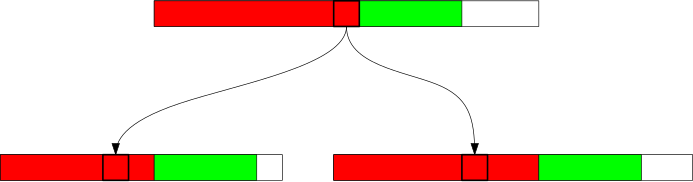
\includegraphics[width=3.5in]{pics/finishedBlocks.png}
  \caption[Blocks that can be safely garbage collected.]{Finished blocks are shown with red color and unfinished blocks are shown with green color. All the subblocks of a finished block are also finished.}
  \label{fig::finishedBlock}
\end{figure}
